\documentclass[11pt,letterpaper]{article}

\usepackage[margin=1in]{geometry}
\usepackage{amsmath,amssymb,amsthm}
\usepackage{algorithm}
\usepackage{algpseudocode}
\usepackage{booktabs}
\usepackage{tikz}
\usetikzlibrary{matrix,positioning,arrows.meta}
\usepackage{hyperref}
\usepackage{xcolor}

% Custom colors
\definecolor{highlight}{RGB}{0,100,150}
\definecolor{example}{RGB}{50,120,50}

% Theorem environments
\theoremstyle{definition}
\newtheorem{definition}{Definition}[section]
\newtheorem{example}{Example}[section]
\theoremstyle{plain}
\newtheorem{theorem}{Theorem}[section]
\newtheorem{lemma}[theorem]{Lemma}
\theoremstyle{remark}
\newtheorem*{remark}{Remark}
\newtheorem*{insight}{Key Insight}

% Convenience macros
\newcommand{\GF}{\mathrm{GF}}
\newcommand{\Hilb}{\mathcal{H}}
\newcommand{\Zn}{\mathbb{Z}_n}
\newcommand{\xmark}{\textcolor{red}{\ding{55}}}
\newcommand{\cmark}{\textcolor{green}{\ding{51}}}

\title{Understanding Hilbert Curves Through Linear Algebra\\[0.5em]
\large From Bit-Fiddling to Group Theory}
\author{}
\date{}

\begin{document}
\maketitle

\begin{abstract}
The Hilbert curve is a beautiful mathematical object that maps a one-dimensional
index to points in multi-dimensional space while preserving locality. Traditional
implementations rely on intricate bit manipulations that obscure the underlying
structure. This document shows how recasting the Hilbert curve in the language of
linear algebra over $\GF(2)$ (the two-element field) reveals that the algorithm
is just a composition of simple, well-understood operations. This perspective not
only clarifies correctness proofs but also unlocks efficient parallel implementations.
\end{abstract}

\tableofcontents
\newpage

%%%%%%%%%%%%%%%%%%%%%%%%%%%%%%%%%%%%%%%%%%%%%%%%%%%%%%%%%%%%%%%%%%%%%%%%%%%%%%%
\section{What Is a Hilbert Curve?}
%%%%%%%%%%%%%%%%%%%%%%%%%%%%%%%%%%%%%%%%%%%%%%%%%%%%%%%%%%%%%%%%%%%%%%%%%%%%%%%

\subsection{The Problem}

Imagine you have a large $n$-dimensional grid of points---say, pixels in an image
($n=2$) or voxels in a 3D volume ($n=3$). You want to assign each point a unique
integer \emph{index} such that:

\begin{enumerate}
    \item Every point gets exactly one index (it's a bijection).
    \item Points with consecutive indices are \emph{neighbors} in the grid.
\end{enumerate}

The second property is the magic: if you walk through the indices $0, 1, 2, \ldots$,
you trace a path that never ``jumps''---each step moves to an adjacent cell.

\begin{figure}[h]
\centering
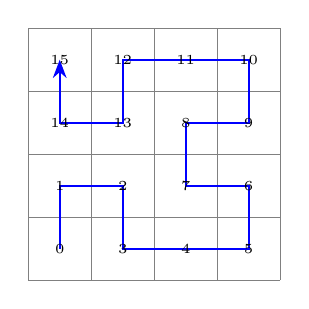
\begin{tikzpicture}[scale=0.8]
    % 4x4 grid
    \draw[gray, thin] (0,0) grid (4,4);

    % Hilbert curve path
    \draw[thick, blue, -{Stealth}]
        (0.5,0.5) -- (0.5,1.5) -- (1.5,1.5) -- (1.5,0.5) --
        (2.5,0.5) -- (3.5,0.5) -- (3.5,1.5) -- (2.5,1.5) --
        (2.5,2.5) -- (3.5,2.5) -- (3.5,3.5) -- (2.5,3.5) --
        (1.5,3.5) -- (1.5,2.5) -- (0.5,2.5) -- (0.5,3.5);

    % Index labels
    \foreach \x/\y/\i in {
        0/0/0, 0/1/1, 1/1/2, 1/0/3,
        2/0/4, 3/0/5, 3/1/6, 2/1/7,
        2/2/8, 3/2/9, 3/3/10, 2/3/11,
        1/3/12, 1/2/13, 0/2/14, 0/3/15
    } {
        \node[font=\tiny] at (\x+0.5, \y+0.5) {\i};
    }
\end{tikzpicture}
\caption{A 2D Hilbert curve on a $4 \times 4$ grid. Numbers show the index;
the blue line shows the path.}
\end{figure}

\subsection{Why Care?}

Hilbert curves are used in:
\begin{itemize}
    \item \textbf{Database indexing:} Store multi-dimensional data (like geographic
    coordinates) in a 1D index while preserving spatial locality.
    \item \textbf{Cache optimization:} Access patterns that follow the Hilbert curve
    have excellent cache behavior.
    \item \textbf{Parallel load balancing:} Divide work among processors by index
    ranges while keeping spatially-related work together.
    \item \textbf{Image processing:} The curve's fractal structure enables
    progressive transmission.
\end{itemize}

\subsection{The Two Operations}

Given a Hilbert curve, we need two operations:
\begin{align*}
    \texttt{encode}: &\quad \text{point } p \mapsto \text{index } h \\
    \texttt{decode}: &\quad \text{index } h \mapsto \text{point } p
\end{align*}

Traditional implementations of these operations involve nested loops, conditional
bit manipulations, and lookup tables. The code is correct but \emph{opaque}---it's
hard to see why it works or how to modify it.

Our goal: rewrite these operations using linear algebra so the structure becomes
transparent.

%%%%%%%%%%%%%%%%%%%%%%%%%%%%%%%%%%%%%%%%%%%%%%%%%%%%%%%%%%%%%%%%%%%%%%%%%%%%%%%
\section{The Vector Space $\GF(2)^n$}
%%%%%%%%%%%%%%%%%%%%%%%%%%%%%%%%%%%%%%%%%%%%%%%%%%%%%%%%%%%%%%%%%%%%%%%%%%%%%%%

\subsection{What Is $\GF(2)$?}

$\GF(2)$ is the simplest possible number system: just $\{0, 1\}$ with arithmetic
modulo 2.

\begin{center}
\begin{tabular}{c|cc}
    $+$ & 0 & 1 \\ \hline
    0 & 0 & 1 \\
    1 & 1 & 0
\end{tabular}
\qquad\qquad
\begin{tabular}{c|cc}
    $\times$ & 0 & 1 \\ \hline
    0 & 0 & 0 \\
    1 & 0 & 1
\end{tabular}
\end{center}

Notice: addition in $\GF(2)$ is exactly XOR ($\oplus$), and every element is its
own inverse ($1 + 1 = 0$).

\subsection{Vectors Over $\GF(2)$}

An element of $\GF(2)^n$ is an $n$-tuple of bits:
\[
    v = (v_0, v_1, \ldots, v_{n-1}), \quad v_j \in \{0, 1\}
\]

We can identify this with an $n$-bit integer:
\[
    v \leftrightarrow \sum_{j=0}^{n-1} v_j \cdot 2^j
\]

\begin{example}
For $n = 3$:
\begin{align*}
    (1, 0, 1) &\leftrightarrow 1 \cdot 2^0 + 0 \cdot 2^1 + 1 \cdot 2^2 = 5 \\
    (0, 1, 1) &\leftrightarrow 0 \cdot 2^0 + 1 \cdot 2^1 + 1 \cdot 2^2 = 6
\end{align*}
\end{example}

\textbf{Vector addition} is componentwise XOR:
\[
    (1, 0, 1) + (0, 1, 1) = (1 \oplus 0, 0 \oplus 1, 1 \oplus 1) = (1, 1, 0)
\]
As integers: $5 \oplus 6 = 3$. \checkmark

\subsection{Why This Matters}

The grid points we care about are exactly $\GF(2)^n$ when the grid has $2^m$ points
per axis. Each coordinate is an $m$-bit number, and at each ``level'' of the Hilbert
recursion, we extract one bit from each coordinate to form an $n$-bit vector.

\begin{insight}
The Hilbert curve operates on $\GF(2)^n$ vectors. All the bit manipulations in
traditional code are really just linear algebra over this field.
\end{insight}

%%%%%%%%%%%%%%%%%%%%%%%%%%%%%%%%%%%%%%%%%%%%%%%%%%%%%%%%%%%%%%%%%%%%%%%%%%%%%%%
\section{Linear Operators on $\GF(2)^n$}
%%%%%%%%%%%%%%%%%%%%%%%%%%%%%%%%%%%%%%%%%%%%%%%%%%%%%%%%%%%%%%%%%%%%%%%%%%%%%%%

A \emph{linear operator} on $\GF(2)^n$ is a function $A: \GF(2)^n \to \GF(2)^n$
that can be represented as matrix multiplication (over $\GF(2)$).

The Hilbert curve uses three key operators. Let's meet them.

\subsection{Cyclic Rotation $\rho$}

The rotation operator shifts all components one position to the right, with
wraparound:
\[
    (\rho \, v)_j = v_{(j-1) \bmod n}
\]

\begin{example}
For $n = 3$:
\[
    \rho(v_0, v_1, v_2) = (v_2, v_0, v_1)
\]
As a matrix:
\[
    \rho = \begin{pmatrix}
        0 & 0 & 1 \\
        1 & 0 & 0 \\
        0 & 1 & 0
    \end{pmatrix}
\]
\end{example}

\textbf{Properties:}
\begin{itemize}
    \item $\rho^n = I$ (rotating $n$ times returns to the start)
    \item $\rho^{-1} = \rho^{n-1}$ (rotate left = rotate right $n-1$ times)
    \item $\rho$ is a \emph{permutation matrix}---it just shuffles components
\end{itemize}

\subsection{The Gray Code $G$}

The Gray code operator transforms a binary number so that consecutive integers
differ in exactly one bit:
\[
    G(v)_j = \begin{cases}
        v_j \oplus v_{j+1} & j < n-1 \\
        v_{n-1} & j = n-1
    \end{cases}
\]

\begin{example}
For $n = 3$:
\[
    G = \begin{pmatrix}
        1 & 1 & 0 \\
        0 & 1 & 1 \\
        0 & 0 & 1
    \end{pmatrix}
    = I + N
\]
where $N$ is the nilpotent ``shift up'' matrix.
\end{example}

\textbf{The Gray code sequence:}
\begin{center}
\begin{tabular}{c|c|c}
    $i$ & binary & $G(i)$ \\ \hline
    0 & 000 & 000 \\
    1 & 001 & 001 \\
    2 & 010 & 011 \\
    3 & 011 & 010 \\
    4 & 100 & 110 \\
    5 & 101 & 111 \\
    6 & 110 & 101 \\
    7 & 111 & 100
\end{tabular}
\end{center}

Notice: each row differs from the next in exactly one bit! This is the key property
that makes Hilbert curves work.

\subsection{The Inverse Gray Code $G^{-1}$}

Since $G$ is an invertible matrix, we can compute $G^{-1}$:
\[
    (G^{-1} v)_j = \bigoplus_{k=j}^{n-1} v_k
\]
This is the XOR of all bits from position $j$ to the end---a ``prefix XOR from the right.''

\begin{example}
For $n = 3$:
\[
    G^{-1} = \begin{pmatrix}
        1 & 1 & 1 \\
        0 & 1 & 1 \\
        0 & 0 & 1
    \end{pmatrix}
\]
This is upper triangular with all 1s on and above the diagonal.
\end{example}

\subsection{Why $G$ Is Central}

The Gray code is the heart of the Hilbert curve. Its property---consecutive values
differ in one bit---means consecutive values are \emph{adjacent vertices of a
hypercube}. This adjacency is what makes the Hilbert curve continuous.

\begin{insight}
The Gray code $G$ is a \textbf{linear operator}. All the ``bit twiddling'' to
compute Gray codes is just matrix multiplication over $\GF(2)$.
\end{insight}

%%%%%%%%%%%%%%%%%%%%%%%%%%%%%%%%%%%%%%%%%%%%%%%%%%%%%%%%%%%%%%%%%%%%%%%%%%%%%%%
\section{The Affine Transform $T_{e,d}$}
%%%%%%%%%%%%%%%%%%%%%%%%%%%%%%%%%%%%%%%%%%%%%%%%%%%%%%%%%%%%%%%%%%%%%%%%%%%%%%%

The Hilbert curve needs one more ingredient: a way to ``reorient'' the Gray code
for different subcubes. This is the transform $T_{e,d}$.

\subsection{Definition}

For $e \in \GF(2)^n$ (the ``entry point'') and $d \in \Zn$ (the ``direction''),
define:
\[
    T_{e,d}(v) = \rho^{d+1}(v \oplus e)
\]

This is an \emph{affine} map: XOR by $e$ (translation), then rotate.

\subsection{What It Does}

$T_{e,d}$ takes the standard Gray code ordering and ``reorients'' it:
\begin{itemize}
    \item XOR by $e$: shifts which corner we start from
    \item Rotate by $d+1$: changes which axis we traverse first
\end{itemize}

\subsection{The Inverse}

\[
    T_{e,d}^{-1}(w) = \rho^{-(d+1)}(w) \oplus e
\]

Just undo in reverse order: rotate back, then XOR.

\subsection{Key Property}

\begin{lemma}
$T_{e,d}$ preserves adjacency: if $u$ and $v$ differ in one bit, so do
$T_{e,d}(u)$ and $T_{e,d}(v)$.
\end{lemma}

\begin{proof}
XOR by a constant preserves bit differences. Rotation just moves which bit
position the difference is in.
\end{proof}

\begin{insight}
Since $T_{e,d}$ preserves adjacency, $T_{e,d}^{-1} \circ G$ is still a Gray code---a
reoriented one that starts at a different corner and traverses axes in a different
order.
\end{insight}

%%%%%%%%%%%%%%%%%%%%%%%%%%%%%%%%%%%%%%%%%%%%%%%%%%%%%%%%%%%%%%%%%%%%%%%%%%%%%%%
\section{The Hilbert Group $\Hilb$}
%%%%%%%%%%%%%%%%%%%%%%%%%%%%%%%%%%%%%%%%%%%%%%%%%%%%%%%%%%%%%%%%%%%%%%%%%%%%%%%

Now we reach the key algebraic insight: the Hilbert curve's ``state'' forms a
\emph{group}.

\subsection{The State}

As the Hilbert algorithm processes each level of the recursion, it maintains a
state $(e, d)$:
\begin{itemize}
    \item $e \in \GF(2)^n$: the entry point of the current subcube
    \item $d \in \Zn$: the current traversal direction
\end{itemize}

\subsection{The Group Structure}

The set of all states forms the \textbf{Hilbert group}:
\[
    \Hilb = \GF(2)^n \rtimes \Zn
\]

This is a \emph{semidirect product}. The group operation is:
\[
    (e_1, \delta_1) \cdot (e_2, \delta_2) = (e_1 \oplus \rho^{-\delta_1}(e_2), \;
    \delta_1 + \delta_2 \mod n)
\]

where we use $\delta = d + 1$ for cleaner formulas.

\textbf{Group properties:}
\begin{itemize}
    \item Identity: $(0, 0)$
    \item Inverse: $(e, \delta)^{-1} = (\rho^{\delta}(e), -\delta)$
    \item Size: $|\Hilb| = n \cdot 2^n$
\end{itemize}

\begin{example}
For $n = 2$: $|\Hilb| = 2 \cdot 4 = 8$ states.

For $n = 3$: $|\Hilb| = 3 \cdot 8 = 24$ states.
\end{example}

\subsection{Why a Group?}

The group operation captures how orientations \emph{compose}. When you enter a
subcube with state $S_1$ and that subcube has relative orientation $S_2$, the
combined orientation is $S_1 \cdot S_2$.

This is the insight that transforms the Hilbert algorithm from ``iterative state
update'' to ``group multiplication.''

%%%%%%%%%%%%%%%%%%%%%%%%%%%%%%%%%%%%%%%%%%%%%%%%%%%%%%%%%%%%%%%%%%%%%%%%%%%%%%%
\section{The Generator $\mu$}
%%%%%%%%%%%%%%%%%%%%%%%%%%%%%%%%%%%%%%%%%%%%%%%%%%%%%%%%%%%%%%%%%%%%%%%%%%%%%%%

\subsection{Definition}

The \textbf{generator} $\mu: \{0, \ldots, 2^n - 1\} \to \Hilb$ maps each
``digit'' (child index) to its relative orientation:
\[
    \mu(w) = (e(w), d(w) + 1)
\]

where $e(w)$ and $d(w)$ are Hamilton's entry point and direction functions.

\subsection{What $\mu$ Encodes}

The generator encapsulates the \emph{geometry} of the Hilbert curve:
\begin{itemize}
    \item How each of the $2^n$ children of a hypercube is oriented
    \item The ``gluing conditions'' that make consecutive children adjacent
\end{itemize}

Different choices of $\mu$ give different space-filling curves. The Hilbert curve
is special because its $\mu$ satisfies:
\begin{enumerate}
    \item The curve starts at corner $0$ and exits at corner $\mathbf{e}_{n-1}$
    \item Child $i$'s exit is adjacent to child $(i+1)$'s entry
\end{enumerate}

\subsection{Example: $n = 2$}

\begin{center}
\begin{tabular}{c|c|c|c}
    $w$ & $e(w)$ & $d(w)$ & $\mu(w)$ \\ \hline
    0 & 0 & 0 & $(0, 1)$ \\
    1 & 0 & 1 & $(0, 0)$ \\
    2 & 0 & 1 & $(0, 0)$ \\
    3 & 3 & 0 & $(3, 1)$
\end{tabular}
\end{center}

Notice: $\mu(1) = \mu(2) = (0, 0)$ is the \emph{identity}! These children don't
change the state at all.

%%%%%%%%%%%%%%%%%%%%%%%%%%%%%%%%%%%%%%%%%%%%%%%%%%%%%%%%%%%%%%%%%%%%%%%%%%%%%%%
\section{The Algorithm: Loop as Scan}
%%%%%%%%%%%%%%%%%%%%%%%%%%%%%%%%%%%%%%%%%%%%%%%%%%%%%%%%%%%%%%%%%%%%%%%%%%%%%%%

Now we can state the Hilbert algorithm in its algebraic form.

\subsection{The Traditional View}

A point $p$ with $m$ bits per coordinate is processed level by level:
\begin{enumerate}
    \item Extract the ``level label'' $\ell_s$ (one bit from each coordinate)
    \item Transform it using current state: $w_s = G^{-1}(T_{e,d}(\ell_s))$
    \item Update state: $(e, d) \leftarrow (e, d) \cdot \mu(w_s)$
    \item Repeat for next level
\end{enumerate}

This looks like a sequential loop with mutable state.

\subsection{The Algebraic View}

\begin{insight}
The loop is a \textbf{scan} (parallel prefix) over the group $\Hilb$.
\end{insight}

For \textbf{decoding} (index $\to$ point):
\begin{enumerate}
    \item Extract digits $(w_m, w_{m-1}, \ldots, w_1)$ from index
    \item \textbf{Map:} Convert each digit to a group element via $\mu$
    \item \textbf{Scan:} Compute prefix products to get all states $S_1, S_2, \ldots$
    \item \textbf{Map:} Apply $\Phi^{-1}_{S_k}(w_k) = T^{-1}_{S_k}(G(w_k))$ at each level
    \item Reassemble level labels into coordinates
\end{enumerate}

\subsection{Decoding Pseudocode}

\begin{algorithm}[H]
\caption{Parallel Hilbert Decoding}
\begin{algorithmic}[1]
\Function{Decode}{$h$}
    \State $W \gets$ extract digits from $h$ \Comment{Parallel: $O(1)$ depth}
    \State $M \gets$ map $\mu$ over $W$ \Comment{Parallel: $O(1)$ depth}
    \State $S \gets$ scan$({\cdot}, (0,1), M)$ \Comment{Parallel: $O(\log m)$ depth}
    \State $L \gets$ zipWith$(\Phi^{-1}, S, W)$ \Comment{Parallel: $O(1)$ depth}
    \State \Return reassemble$(L)$
\EndFunction
\end{algorithmic}
\end{algorithm}

\textbf{Total depth: $O(\log m)$} --- logarithmic in the number of bits!

\subsection{Why Decoding Parallelizes}

The key is that the group operation is \emph{associative}:
\[
    (a \cdot b) \cdot c = a \cdot (b \cdot c)
\]

Any associative operation can be computed with a parallel scan in $O(\log n)$ depth.
This is a fundamental result from parallel algorithms.

%%%%%%%%%%%%%%%%%%%%%%%%%%%%%%%%%%%%%%%%%%%%%%%%%%%%%%%%%%%%%%%%%%%%%%%%%%%%%%%
\section{Encoding: The Clever Trick}
%%%%%%%%%%%%%%%%%%%%%%%%%%%%%%%%%%%%%%%%%%%%%%%%%%%%%%%%%%%%%%%%%%%%%%%%%%%%%%%

\subsection{The Apparent Problem}

Encoding (point $\to$ index) seems harder. At each level:
\[
    w_k = \Phi_{S_k}(\ell_k) = G^{-1}(T_{S_k}(\ell_k))
\]

But $S_k$ depends on $w_1, \ldots, w_{k-1}$, which we haven't computed yet!

This is a \textbf{triangular dependency}:
\[
    S_{k+1} = S_k \cdot \mu(w_k), \quad w_k = \Phi_{S_k}(\ell_k)
\]

It looks inherently sequential.

\subsection{The Solution: Function Composition}

Here's the trick: instead of working with \emph{states}, work with
\emph{transition functions}.

For each level label $\ell$, define the function $f_\ell: \Hilb \to \Hilb$:
\[
    f_\ell(S) = S \cdot \mu(\Phi_S(\ell))
\]

This is ``given state $S$, compute the digit, then update the state.''

\begin{insight}
Function composition is associative! We can compute $f_m \circ f_{m-1} \circ \cdots
\circ f_1$ with a parallel scan.
\end{insight}

\subsection{How It Works}

Each function $f_\ell$ can be represented as a \textbf{lookup table}: for each of
the $|\Hilb|$ possible input states, store the output state.

Composing two functions is just:
\[
    (f \circ g)[S] = f[g[S]]
\]

This is $O(|\Hilb|)$ work per composition.

\subsection{Parallel Encoding Algorithm}

\begin{algorithm}[H]
\caption{Parallel Hilbert Encoding}
\begin{algorithmic}[1]
\Function{Encode}{$p$}
    \State $L \gets$ extract level labels from $p$ \Comment{Parallel: $O(1)$ depth}
    \State $f \gets$ map buildTable over $L$ \Comment{Parallel: $O(|\Hilb|)$ work each}
    \State $F \gets$ scan$(\circ, \mathrm{id}, f)$ \Comment{Parallel: $O(\log m)$ depth}
    \For{$k = 1$ to $m$} \textbf{parallel}
        \State $S_k \gets F_{k-1}(S_{\text{initial}})$
        \State $w_k \gets \Phi_{S_k}(\ell_k)$
    \EndFor
    \State \Return pack$(W)$
\EndFunction
\end{algorithmic}
\end{algorithm}

\textbf{Total depth: $O(\log m)$} --- same as decoding!

\subsection{The Cost}

\begin{center}
\begin{tabular}{l|cc}
    & Sequential & Parallel \\ \hline
    Depth & $O(m)$ & $O(\log m)$ \\
    Work & $O(m)$ & $O(m \cdot n \cdot 2^n)$ \\
    Space & $O(1)$ & $O(m \cdot n \cdot 2^n)$
\end{tabular}
\end{center}

We trade off more total work for much less depth. This is exactly what GPUs are
designed for.

\subsection{When Is This Practical?}

The lookup table size is $|\Hilb| = n \cdot 2^n$:

\begin{center}
\begin{tabular}{c|c|l}
    $n$ & $|\Hilb|$ & Notes \\ \hline
    2 & 8 & Trivial \\
    3 & 24 & Easy \\
    4 & 64 & Fits in registers \\
    5 & 160 & Comfortable \\
    6 & 384 & Still practical \\
    7 & 896 & Getting large \\
    8 & 2048 & Possible but expensive
\end{tabular}
\end{center}

For typical applications ($n \leq 6$), this is very practical.

%%%%%%%%%%%%%%%%%%%%%%%%%%%%%%%%%%%%%%%%%%%%%%%%%%%%%%%%%%%%%%%%%%%%%%%%%%%%%%%
\section{GPU Implementation}
%%%%%%%%%%%%%%%%%%%%%%%%%%%%%%%%%%%%%%%%%%%%%%%%%%%%%%%%%%%%%%%%%%%%%%%%%%%%%%%

\subsection{Why GPUs?}

GPUs excel at:
\begin{itemize}
    \item Massive parallelism (thousands of threads)
    \item SIMD operations (same operation on many data elements)
    \item High memory bandwidth
\end{itemize}

But they struggle with:
\begin{itemize}
    \item Sequential dependencies
    \item Irregular control flow (branches)
    \item Low parallelism
\end{itemize}

The algebraic Hilbert formulation is perfect for GPUs.

\subsection{Batch Processing}

In practice, you rarely encode/decode a single point. You have millions of points.

\textbf{Outer parallelism:} Process many points in parallel. Each thread handles one
point. This is embarrassingly parallel.

\textbf{Inner parallelism:} Within each point, use the scan-based algorithm to
process levels in $O(\log m)$ depth.

\subsection{Implementation Strategy}

\subsubsection{Decoding (Index $\to$ Point)}

\begin{enumerate}
    \item \textbf{Precompute $\mu$:} Store the generator as a lookup table in shared
    memory or registers. Size: $2^n$ entries of $(e, \delta)$ pairs.

    \item \textbf{Per-point parallel scan:} Use warp-level primitives
    (\texttt{\_\_shfl\_*} on NVIDIA) to compute the prefix product of group elements.

    \item \textbf{Apply transforms:} Each thread computes $T^{-1}_{S_k}(G(w_k))$ for
    its assigned level. Rotation and XOR are single instructions.
\end{enumerate}

\subsubsection{Encoding (Point $\to$ Index)}

\begin{enumerate}
    \item \textbf{Precompute transition tables:} For each possible level label
    $\ell \in \GF(2)^n$, precompute the function $f_\ell$ as a table of size
    $|\Hilb|$. Total: $2^n$ tables of $n \cdot 2^n$ entries each.

    \item \textbf{Select tables:} Based on the level labels of the input point,
    select the appropriate function tables.

    \item \textbf{Parallel scan on functions:} Compose the function tables using
    warp-level scan.

    \item \textbf{Evaluate and extract digits:} Apply the composed functions to
    get states, then compute digits.
\end{enumerate}

\subsection{Memory Layout}

For best GPU performance:

\begin{itemize}
    \item \textbf{Coalesced access:} Store points in structure-of-arrays format
    (all $x$-coordinates together, all $y$-coordinates together, etc.)

    \item \textbf{Shared memory:} Keep lookup tables in shared memory for fast
    access within a thread block.

    \item \textbf{Registers:} For small $n$, the entire state and intermediate
    values fit in registers.
\end{itemize}

\subsection{Complexity Summary}

For $N$ points with $m$ bits per coordinate in $n$ dimensions:

\begin{center}
\begin{tabular}{l|cc}
    & CPU (sequential) & GPU (parallel) \\ \hline
    Decode & $O(N \cdot m)$ & $O(N \cdot m / P + \log m)$ \\
    Encode & $O(N \cdot m)$ & $O(N \cdot m \cdot n \cdot 2^n / P + \log m)$
\end{tabular}
\end{center}

where $P$ is the number of parallel processors.

The key insight: the $\log m$ term is the \emph{depth}, which determines latency.
The $N/P$ term is the \emph{throughput}. GPUs have large $P$, so the throughput
term dominates for large $N$.

\subsection{When to Use This}

The parallel algorithm wins when:
\begin{itemize}
    \item You have many points to process (large $N$)
    \item Latency matters (real-time applications)
    \item You're already on a GPU (avoid CPU-GPU transfer overhead)
\end{itemize}

The sequential algorithm might still win for:
\begin{itemize}
    \item Single-point queries
    \item Very high dimensions ($n > 8$)
    \item Memory-constrained environments
\end{itemize}

%%%%%%%%%%%%%%%%%%%%%%%%%%%%%%%%%%%%%%%%%%%%%%%%%%%%%%%%%%%%%%%%%%%%%%%%%%%%%%%
\section{Summary: What We Gained}
%%%%%%%%%%%%%%%%%%%%%%%%%%%%%%%%%%%%%%%%%%%%%%%%%%%%%%%%%%%%%%%%%%%%%%%%%%%%%%%

\subsection{Conceptual Clarity}

By recasting the Hilbert curve in terms of $\GF(2)^n$ linear algebra:

\begin{center}
\begin{tabular}{l|l}
    \textbf{Old view} & \textbf{New view} \\ \hline
    Bit manipulation & Linear operators ($G$, $\rho$) \\
    Mutable state & Group elements in $\Hilb$ \\
    Sequential loop & Parallel scan \\
    Magic formulas & Group multiplication \\
    ``It works because Hamilton said so'' & Algebraic proof
\end{tabular}
\end{center}

\subsection{Practical Benefits}

\begin{enumerate}
    \item \textbf{Correctness:} Proofs become algebraic identities instead of
    case-by-case bit analysis.

    \item \textbf{Parallelism:} Both encoding and decoding achieve $O(\log m)$ depth.

    \item \textbf{Modularity:} The geometry ($\mu$) is separate from the algebra
    ($\Hilb$) and the algorithm (scan).

    \item \textbf{Generalization:} Want a different space-filling curve? Just change
    $\mu$, keeping everything else the same.
\end{enumerate}

\subsection{The Deep Insight}

The Hilbert curve looks sequential because traditional presentations focus on
\emph{state values}. But the values aren't what matter---what matters is the
\emph{function from initial state to final state}.

Functions compose associatively. That's why we can parallelize.

This is a general principle: many ``inherently sequential'' algorithms become
parallel when you lift from values to functions. The Hilbert curve is a beautiful
example.

\vspace{1em}
\hrule
\vspace{1em}

\begin{center}
\textit{The Hilbert curve's ``inherently sequential'' reputation is a myth.\\
The algebraic structure unlocks parallelism.}
\end{center}

\end{document}
